\chapter{Navrhování algoritmů}

\section{Časová a prostorová složitost algoritmů}
	Abychom mohli porovnávat algoritmy, řešící stejný problém, mezi sebou a rozhodnout se kdy který algoritmus použít, slouží nám k tomuto účelu základní dvě míry pro porovnání.
\begin{itemize}
	\item časová složitost
	\item prostorová složitost
\end{itemize}
	Časová složitost vyjadřuje jak dlouho bude výpočet podle daného algoritmu trvat, obdobně prostorová složitost nám vyjadřuje kolik prostoru, tedy paměti, danému algoritmu budeme muset poskytnout pro výpočet. Je očividné že vyjadřovat časovou složitost v sekundách a prostorovou v bytech by vzhledem k různému hardwaru, či různé implementaci nebylo příliš vhodné. Pro popis složitosti algoritmu tedy zavádíme pojem \textit{Asymptotická složitost}.
	
\subsection{Asymptotická složitost}
	Asymptotická složitost se vyjadřuje jako matematická funkce, popisující závislost využití paměťového prostoru nebo výpočetního výkonu na velikosti vstupních dat $N$. Důležité je že tato funkce je neklesající a vyjadřujeme ji pouze jako třídu složitosti, tedy typ funkce a ne jako přesné vyjádření. Pro příklad funkce $\mathcal{O} (1000N^2) $ nebo $\mathcal{O} (N^2 + 1000N)$ jsou třídy složitosti $\mathcal{O} (N^2)$. Tedy zanedbáváme multiplikativní konstantu, aditivní konstantu a nižší řády funkce, protože nás zajíma jak se bude měnit časová náročnost s velikostí vstupních dat.
	Tím že zanedbáváme multiplikativní, aditivní konstantu a nižší řády funkce, může se vyskytnout případ kdy algoritmus s horší asymptotickou časovou složitostí proběhne rychleji než algoritmus s lepší asymptotickou časovou složitostí. Máme ovšem jistotu že existuje vstup o velikosti $N_0$, kde toto přestane platit. Při praktickém použití toto může nastat v případě, kdy asymptoticky rychlejší algoritmus má složitější implementaci a prostředky vynaložené na režiji převyšují výhody algoritmu. [něco citovat]
	
\begin{figure}[h]
  \centering
  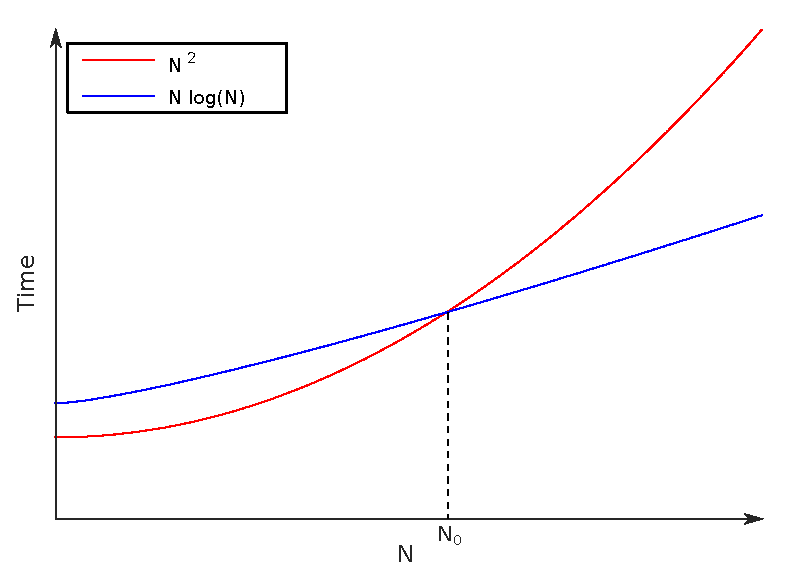
\includegraphics[width=7.5cm]{./pictures/3/time_complexity.pdf}
  \caption{Graf znázorňující průběh algoritmu v závislosti na $N$}
  \label{fig:3-time_complexity}
\end{figure}
	
	
	 Pro vyjádření časové složitosti můžeme využít různé varianty.
\begin{itemize}
	\item Horní odhad složitosti - $\mathcal{O} (f(N))$
	\item Průměrná složitost - $\Theta (f(N))$
	\item Dolní odhad složitosti - $\Omega (f(N))$
\end{itemize}	
	Nejčastěji využívaný odhad je takzvaná \textit{Omikron notace}, která vyjadřuje horní odhad, tedy nejhorší možný případ jakým se může algoritmus chovat. V tomto případě máme jistotu že algoritmus bude asymptoticky probíhat stejně rychle nebo rychleji v případě časové složitosti. V některých případech se vyplatí uvádět i průměrnou složitost, tedy složitost, která nastává při nějakém náhodném rozložení vstupních dat. Tato situace pak lépe vystihuje praktické použití algoritmu, ale nemáme jistotu že se bude chovat asymptoticky hůře. Poslední variantou je dolní odhad složitosti, který nám naopak vyjadřuje že algoritmus se bude chovat stejně nebo hůře než je uvedeno.
	
\subsection{Stanovení časové složitosti}
	[Doplnit] Časovou složitost algoritmu můžeme stanovit matematickou analýzou nebo empiricky. U jednoduchých algoritmů většinou není problém stanovit složitost
	
	
	
	
\section{Metody návrhů algoritmů ve výpočetní geometrii}
	Abychom byli schopni porozumět různým algoritmům, nebo navrhnout nový algoritmus pro různé operace ve výpočetní geometrii, je dobré seznámit se s často využívanými metodami, používané v algoritmech výpočetní geometrie. Metody návrhů alogritmů neřeší konkrétní problém, ale pouze obecný postup jak se při hledání řešení chovat.

\subsection{Metoda hrubé síly}
	Patří k nejjednodušším metodám algoritmizace. Jak vyplývá z názvu, v této metodě budeme postupovat hrubou silou, tedy v praxi to znamená že algoritmus bude zkoušet všechny možné kombinace řešení. Mezi výhody patří jednoduchá implementace a snadné porozumění algoritmu, které se často shoduje s definicí výsledku. Tyto algoritmy lze využívat zpravidla pro malé vstupní množiny, nebo pro ověření správnosti výsledku. V praxi lze algoritmy využít i jako doplněk složitějších algoritmů, kde by režije, jako je volání funkcí nebo vytváření objektů, zabralo více času než na tuto malou množinu použít algoritmus hrubé síly.
	
\subsection{Rozděl a panuj}
	Nejen ve výpočetní geometrii je známá a hojně používaná metoda \textit{rozděl a panuj}, známá také pod anglickým názvem \textit{divide and conquer}. Paradigma je založeno na rekurzivním rozdělování problému na dvě či více částí, stejného nebo podobného typu, dokud nebudeme schopni problém jednoduše vyřešit. Řešení dílčích problémů se pak spojuje a získá se řešení původního problému. Metoda \textit{rozděl a panuj} je vhodná pro paralelní zpracování, kde pří každém rozdělení nám vznikají dvě či více částí, které můžeme řešit nezávisle na sobě. \cite{frigo1999cache}
	Do algoritmů této kategorie patří například generalizační algoritmus \textit{Douglas-Peucker} \cite{van1997algorithmic}, který je vhodný svou jednoduchostí na ukázkou metody rozděl a panuj. 
	Na vstupu dostává algoritmus linii, kterou chceme generalizovat a hodnotu vzdálenosti o kterou se generalizovaná linie může maximálně lišit od původní. Funkce vyhledá bod s maximální vzdáleností od úsečky spojující počáteční a koncový bod, který je zároveň vzdálenější než námi zadaná mez, poté se rekurzivně zavolá na dvě úsečky obsahující tento bod. Takto se postupuje do té doby dokud existuje bod s větší vzdáleností než zadaná mez. Po dokončení se řešení složí z jednotlivých  kroků rekurze.

\begin{figure}[h]
    \centering % <-- added
\begin{subfigure}{0.5\textwidth}
  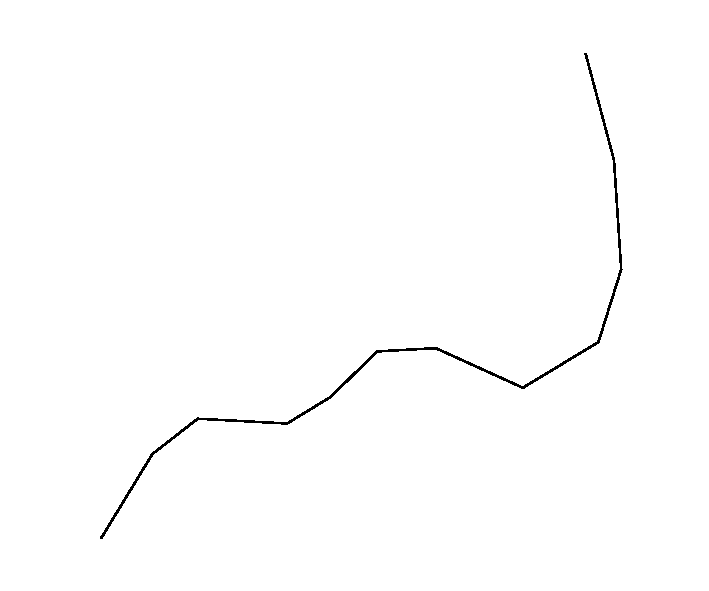
\includegraphics[width=\linewidth]{./pictures/3/douglas-peucker_1.pdf}
  \label{fig:3-douglas-peucker_1}
\end{subfigure}\hfil % <-- added
\begin{subfigure}{0.5\textwidth}
  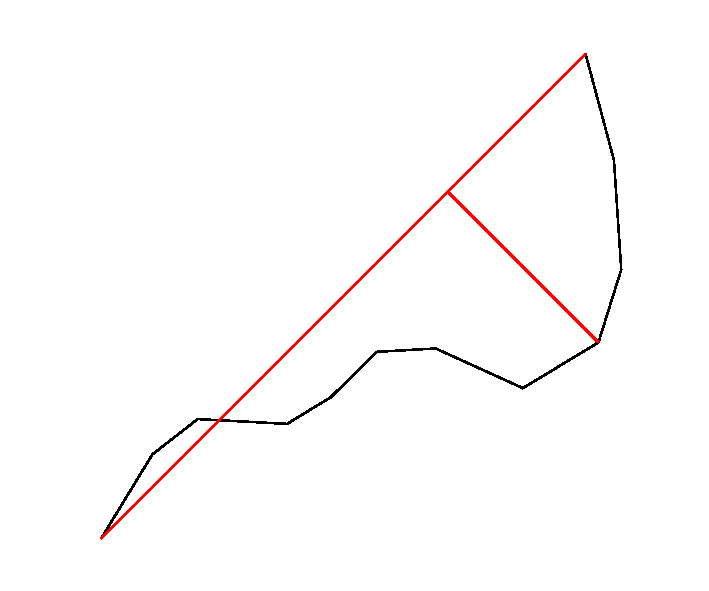
\includegraphics[width=\linewidth]{./pictures/3/douglas-peucker_2.pdf}
  \label{fig:3-douglas-peucker_2}
\end{subfigure}\hfil % <-- added
\begin{subfigure}{0.5\textwidth}
  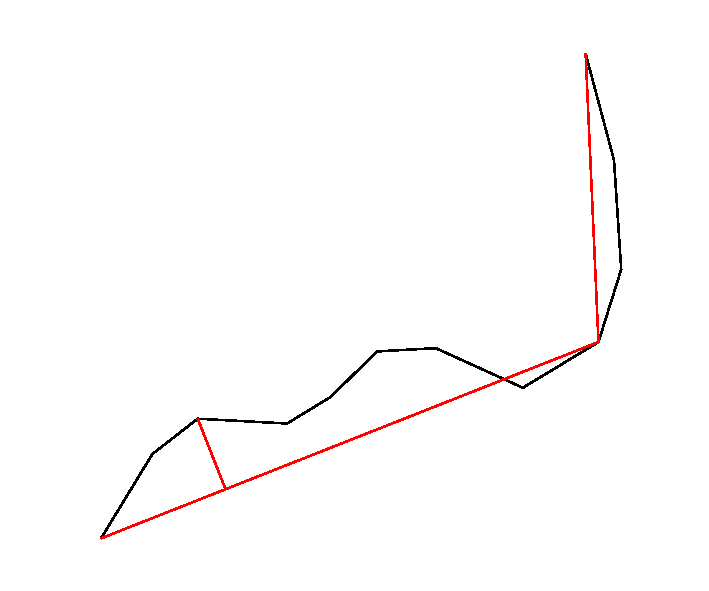
\includegraphics[width=\linewidth]{./pictures/3/douglas-peucker_3.pdf}
  \label{fig:3-douglas-peucker_3}
\end{subfigure}\hfil % <-- added
\begin{subfigure}{0.5\textwidth}
  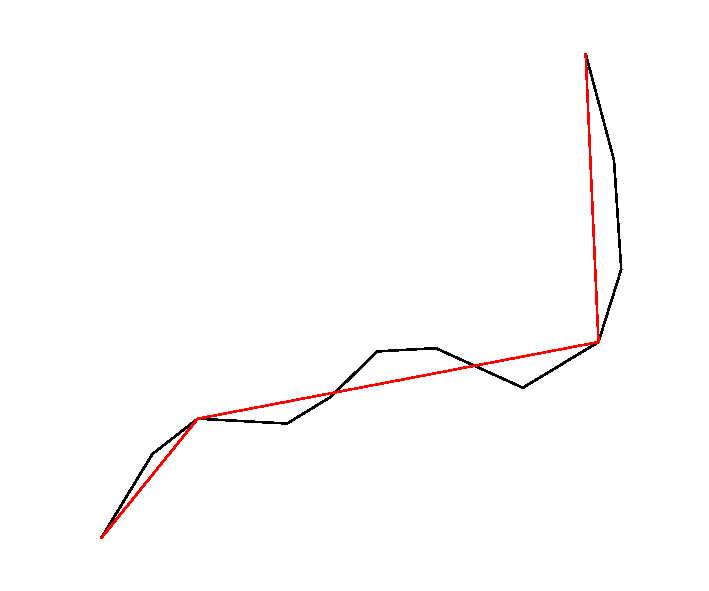
\includegraphics[width=\linewidth]{./pictures/3/douglas-peucker_4.pdf}
  \label{fig:3-douglas-peucker_4}
\end{subfigure}\hfil % <-- added
\caption{Znázornění postupu \textit{Douglas-Peucker} algoritmu pro ukázku metodi \textit{rozděl a panuj}}
\end{figure}
	

\subsection{Zametací přímka}
	Další metoda využívaná výhradně ve výpočetní geometrii je metoda takzvané \textit{zametací přímky}, neboli \textit{sweep line}. Myšlenkou této techniky je procházení setříděných dat. Ve výpočetní geometrii se nejčastěji jedná o průchod bodů seřazených podle jedné ze souřadnic. Pokud takto setříděnou vstupní množinou nedisponujeme, je nutno nejprve data setřídit jedním ze známích třídících algoritmů. Pak lze průchod body vizualizovat, podle implementace, jako svislou přímku pohybující se z leva do prava po množině bodů.
	Tuto metudu využívá například \textit{Bentley-Ottmannův} algoritmus pro nalezení průsečíků množin linií, který je podrobněji popsán v kapitole \ref{chap:reserzepouzivanychalgoritmu}, proto se jím zde nebudeme zabývat.







\subsection{Inkrementální algoritmy}


\subsection{Heuristické algoritmy}

\subsection{Aproximační algoritmy}

\subsection{Hladové algoritmy}

\subsection{Randomizované algoritmy}














